\section{Result}

\begin{figure}[ht] 
\centering
\subfigure[{}]{ 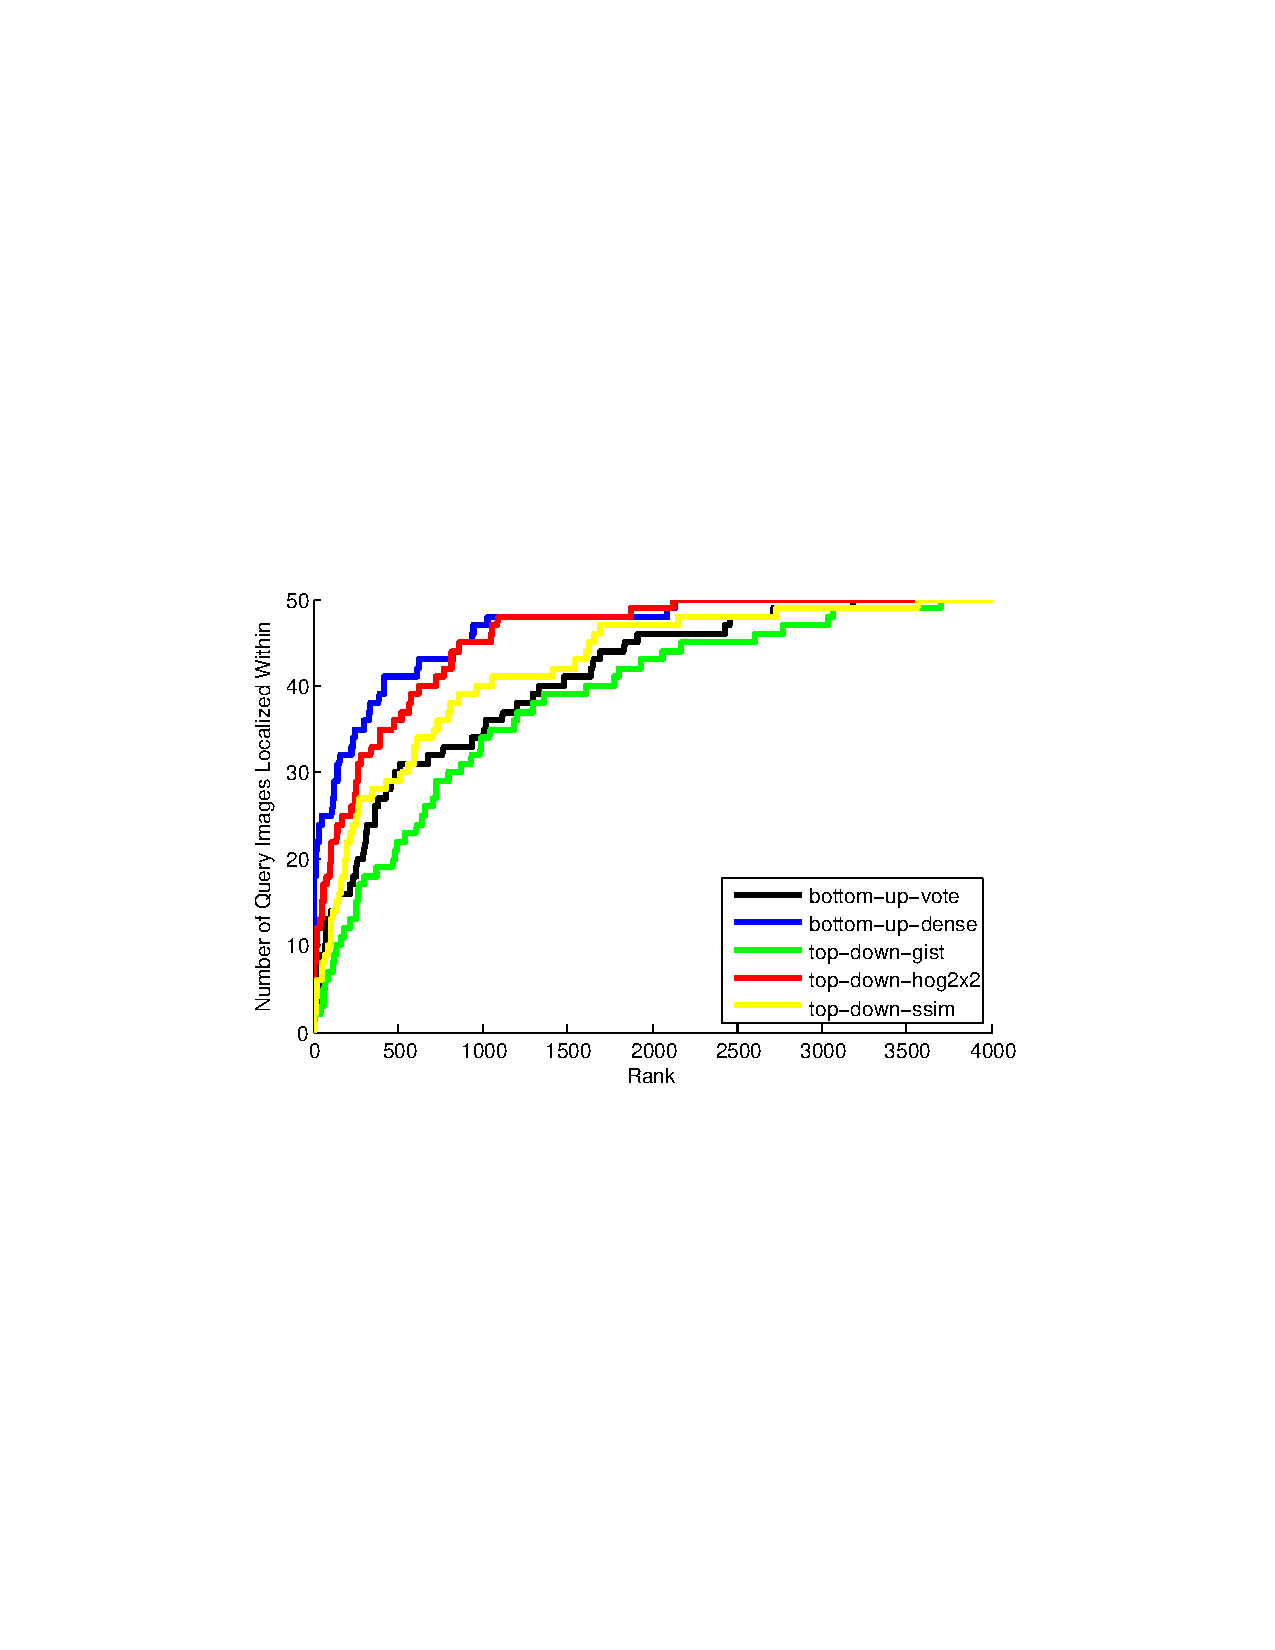
\includegraphics[width=0.5\textwidth]{pictures/result-a} \label{result-a} }
%\subfigure[{}]{ \includegraphics[width=2.5in]{pictures/result-b} \label{result-b} }
\caption[]{\subref{result-a} Example ground level query image and 4 associated aerial images. \subref{result-b} Highlighting the appearance difference in across the two imaging conditions.}
\label{result}
\end{figure}

\label{sec:result}


